%----------------------------------------------------------------------------
%
%	This template was created by
%		Christian Krieg <christian.krieg@alumni.tuwien.ac.at>
%
%	April 2018
%
%----------------------------------------------------------------------------
%
\documentclass[%
	a4paper,
]
{article}
%
%----------------------------------------------------------------------------
%
% Institution
%
%\institution{Institute of Computer Technology}

%
%----------------------------------------------------------------------------
%
% Use the 'Libertine' font type
%
\usepackage{libertine}
\usepackage[T1]{fontenc}
\usepackage[utf8]{inputenc}
%
%----------------------------------------------------------------------------
%
% Set page margins
%
\usepackage{geometry}
\geometry{%
	left   = 2cm,
	right  = 2cm,
	top    = 2cm,
	bottom = 2cm
}
%
%----------------------------------------------------------------------------
%
% Set line spacing
%
\usepackage{setspace}
\setstretch{1}
%----------------------------------------------------------------------------
%
% Use colors
%
\usepackage{xcolor}
\usepackage{colortbl}
%
%----------------------------------------------------------------------------
%
% Define a TODO and a DONE command
%
\newcommand{\todo}[1]{\textcolor{red}{#1}}
\newcommand{\done}[1]{}
%
%----------------------------------------------------------------------------
%
% Use glossaries
%
\usepackage{glossaries}
\makeglossaries
%
% Glossary entries
%
\newglossaryentry{fpga}{
	name = {FPGA},
	description = {Field-programmable gate array},
	text = {FPGA},
	first = {field-programmable gate array (FPGA)},
	plural = {FPGAs},
	firstplural = {field-programmable gate arrays (FPGAs)},
}
%
\newglossaryentry{trng}{
	name = {TRNG},
	description = {True-random number generator},
	text = {TRNG},
	first = {true-random number generator (TRNG)},
	plural = {TRNGs},
	firstplural = {true-random number generators (TRNGs)},
}
%
\newglossaryentry{bcd}{
  name={BCD},
  description={Binary-coded decimal},
  text={BCD},
  first={binary-coded decimal (BCD)},
}
%
\newglossaryentry{hdl}{
  name={HDL},
  description={Hardware description language},
  text={HDL},
  first={hardware description language (HDL)},
  plural={HDLs},
  firstplural={hardware description languages (HDLs)},
}

\newglossaryentry{dicl}{
  name={DIC-Lab},
  description={Course held at TU-Wien on applying digital design techniques},
  text={DIC-Lab},
  first={Digital-Integrated-Circuits Laboratory (DIC-Lab)},
}

\newglossaryentry{bbs}{
  name={BBS},
  description={Blum-Blum-Shub algorithm},
  text={BBS},
  first={Blum-Blum-Shub algorithm (BBS)},
}

\newglossaryentry{prng}{
  name={PRNG},
  description={Pseudo-random number generator (PRNG)},
  text={PRNG},
  first={pseudo-random number generator (PRNG)},
  plural={PRNGs},
  firstplural={pseudo-random number generators (PRNGs)},
}
\newglossaryentry{uart}{
  name={UART},
  description={Universal Asynchronous Receiver Transmitter (UART)},
  text={UART},
  first={Universal Asynchronous Receiver Transmitter (UART)},
  plural={UARTs},
  firstplural={Universal Asynchronous Receiver Transmitters (UARTs)},
}
\newglossaryentry{nist}{
  name={NIST},
  description={National Institute of Standards and Technology (NIST)},
  text={NIST},
  first={National Institute of Standards and Technology (NIST)},
  plural={UARTs},
  firstplural={National Institute of Standards and Technology (NISTs)},
}

%\newglossaryentry{}{
%  name={},
%  description={},
%  text={},
%  first={},
%  plural={},
%  firstplural={},
%}
%
%----------------------------------------------------------------------------
%
% Settings for citations and the bibliography
%
\usepackage[%
	backend     = biber,
	maxbibnames = 99,
	autocite    = footnote,
	citestyle   = verbose-ibid,
	giveninits=true,
]{biblatex}
\bibliography{bib/blake2}
%
%----------------------------------------------------------------------------
%
% For Pseudo code
%
\usepackage{algorithm2e}

%
%----------------------------------------------------------------------------
%
%	TikZ -- TikZ ist kein Zeichenprogramm
%

\usepackage{tikz}
\usepackage{tikz-timing}
\usepackage{etoolbox}
\usetikzlibrary{mindmap}
\usetikzlibrary{shapes}
\usetikzlibrary{arrows}
\usetikzlibrary{decorations}
\usetikzlibrary{shapes.symbols}
\usetikzlibrary{shapes.geometric}
\usetikzlibrary{shapes.multipart}
\usetikzlibrary{positioning}
\usetikzlibrary{patterns}
\usetikzlibrary{calc}
\usetikzlibrary{scopes}         % cf. pgfmanual p.66
\usetikzlibrary{chains}         % cf. pgfmanual p.284
\usetikzlibrary{fit}
\usetikzlibrary{matrix}
\usetikzlibrary{decorations}
\usetikzlibrary{circuits.logic}
\usetikzlibrary{circuits.logic.IEC}
\usetikzlibrary{shapes.gates.logic.IEC}
%\usetikzlibrary{circuits.logic.US}
%\usetikzlibrary{shapes.gates.logic.US}
\usetikzlibrary{circuits.ee}
\usetikzlibrary{circuits.ee.IEC}
\usetikzlibrary{backgrounds}
\usetikzlibrary{automata}
\usetikzlibrary{intersections}
\usetikzlibrary{plotmarks}
\usepgflibrary{fpu}
\usetikzlibrary{decorations.pathreplacing}
%
%----------------------------------------------------------------------------
%
% TikZ shapes
%  
	% D flip-flops (DFFs) and shift register
% Author: Martin Scharrer
%\documentclass[a4paper,landscape]{article}

%\usepackage{pgf,tikz}
%%%<
%\usepackage{verbatim}
%\usepackage[active,tightpage]{preview}
%\PreviewEnvironment{tikzpicture}
%\setlength\PreviewBorder{5pt}%
%%%>

%\begin{comment}
%:Title: D flip-flops and shift register
%
%Example of a custom node shape for drawing  D flip-flops. The shape is used to draw a serial shift
%register. 
%
%\end{comment}
%
%\usetikzlibrary{calc,arrows}
%\usepackage{amsmath}
%\usepackage[left=1cm,right=1cm]{geometry}
%\pagestyle{empty}

\makeatletter

% Data Flip Flip (DFF) shape
\pgfdeclareshape{dff}{
  % The 'minimum width' and 'minimum height' keys, not the content, determine
  % the size
  \savedanchor\northeast{%
    \pgfmathsetlength\pgf@x{\pgfshapeminwidth}%
    \pgfmathsetlength\pgf@y{\pgfshapeminheight}%
    \pgf@x=0.5\pgf@x
    \pgf@y=0.5\pgf@y
  }
  % This is redundant, but makes some things easier:
  \savedanchor\southwest{%
    \pgfmathsetlength\pgf@x{\pgfshapeminwidth}%
    \pgfmathsetlength\pgf@y{\pgfshapeminheight}%
    \pgf@x=-0.5\pgf@x
    \pgf@y=-0.5\pgf@y
  }
  % Inherit from rectangle
  \inheritanchorborder[from=rectangle]

  % Define same anchor a normal rectangle has
  \anchor{center}{\pgfpointorigin}
  \anchor{north}{\northeast \pgf@x=0pt}
  \anchor{east}{\northeast \pgf@y=0pt}
  \anchor{south}{\southwest \pgf@x=0pt}
  \anchor{west}{\southwest \pgf@y=0pt}
  \anchor{north east}{\northeast}
  \anchor{north west}{\northeast \pgf@x=-\pgf@x}
  \anchor{south west}{\southwest}
  \anchor{south east}{\southwest \pgf@x=-\pgf@x}
  \anchor{text}{
    \pgfpointorigin
    \advance\pgf@x by -.5\wd\pgfnodeparttextbox%
    \advance\pgf@y by -.5\ht\pgfnodeparttextbox%
    \advance\pgf@y by +.5\dp\pgfnodeparttextbox%
  }

  % Define anchors for signal ports
  \anchor{D}{
    \pgf@process{\northeast}%
    \pgf@x=-1\pgf@x%
    \pgf@y=.5\pgf@y%
  }
  \anchor{CLK}{
    \pgf@process{\northeast}%
    \pgf@x=-1\pgf@x%
    \pgf@y=-.66666\pgf@y%
  }
  \anchor{CE}{
    \pgf@process{\northeast}%
    \pgf@x=-1\pgf@x%
    \pgf@y=-0.33333\pgf@y%
  }
  \anchor{Q}{
    \pgf@process{\northeast}%
    \pgf@y=.5\pgf@y%
  }
  \anchor{Qn}{
    \pgf@process{\northeast}%
    \pgf@y=-.5\pgf@y%
  }
  \anchor{R}{
    \pgf@process{\northeast}%
    \pgf@x=0pt%
  }
  \anchor{S}{
    \pgf@process{\northeast}%
    \pgf@x=0pt%
    \pgf@y=-\pgf@y%
  }
  % Draw the rectangle box and the port labels
  \backgroundpath{
    % Rectangle box
    \pgfpathrectanglecorners{\southwest}{\northeast}
    % Angle (>) for clock input
    \pgf@anchor@dff@CLK
    \pgf@xa=\pgf@x \pgf@ya=\pgf@y
    \pgf@xb=\pgf@x \pgf@yb=\pgf@y
    \pgf@xc=\pgf@x \pgf@yc=\pgf@y
    \pgfmathsetlength\pgf@x{.75ex} % size depends on font size
    \advance\pgf@ya by \pgf@x
    \advance\pgf@xb by \pgf@x
    \advance\pgf@yc by -\pgf@x
    \pgfpathmoveto{\pgfpoint{\pgf@xa}{\pgf@ya}}
    \pgfpathlineto{\pgfpoint{\pgf@xb}{\pgf@yb}}
    \pgfpathlineto{\pgfpoint{\pgf@xc}{\pgf@yc}}
    \pgfclosepath

    % Draw port labels
    \begingroup
    \tikzset{flip flop/port labels} % Use font from this style
    \tikz@textfont

    \pgf@anchor@dff@D
    \pgftext[left,base,at={\pgfpoint{\pgf@x}{\pgf@y}},x=\pgfshapeinnerxsep]{\raisebox{-0.75ex}{D}}

%    \pgf@anchor@dff@CE
%    \pgftext[left,base,at={\pgfpoint{\pgf@x}{\pgf@y}},x=\pgfshapeinnerxsep]{\raisebox{-0.75ex}{CE}}

    \pgf@anchor@dff@Q
    \pgftext[right,base,at={\pgfpoint{\pgf@x}{\pgf@y}},x=-\pgfshapeinnerxsep]{\raisebox{-.75ex}{Q}}

%    \pgf@anchor@dff@Qn
%    \pgftext[right,base,at={\pgfpoint{\pgf@x}{\pgf@y}},x=-\pgfshapeinnerxsep]{\raisebox{-.75ex}{$\overline{\mbox{Q}}$}}
%
%    \pgf@anchor@dff@R
%    \pgftext[top,at={\pgfpoint{\pgf@x}{\pgf@y}},y=-\pgfshapeinnerysep]{R}
%
%    \pgf@anchor@dff@S
%    \pgftext[bottom,at={\pgfpoint{\pgf@x}{\pgf@y}},y=\pgfshapeinnerysep]{S}
    \endgroup
  }
}

% Key to add font macros to the current font
\tikzset{add font/.code={\expandafter\def\expandafter\tikz@textfont\expandafter{\tikz@textfont#1}}} 

% Define default style for this node
% \tikzset{flip flop/port labels/.style={font=\sffamily\scriptsize}}
%\tikzset{every dff node/.style={draw,minimum width=2cm,minimum 
%height=2.828427125cm,very thick,inner sep=1mm,outer sep=0pt,cap=round,add 
%font=\sffamily}}
\tikzset{flip flop/port labels/.style={font=\tiny}}
\tikzset{every dff node/.style={draw,minimum width=.75cm,minimum 
height=1cm,inner sep=1mm,outer sep=0pt,cap=round,font=\scriptsize}}

\makeatother

%\begin{document}
%
%\begin{tikzpicture}[font=\sffamily,>=triangle 45]
%  \def\N{7}  % Number of Flip-Flops minus one
%
%  % Place FFs
%  \foreach \m in {0,...,\N}
%    \node [shape=dff] (DFF\m) at ($ 3*(\m,0) $) {Bit \#\m};
%
%  % Connect FFs (Q1 with D1, etc.)
%  \def\p{0}  % Used to save the previous number
%  \foreach \m in {1,...,\N} { % Note that it starts with 1, not 0
%    \draw [->] (DFF\p.Q) -- (DFF\m.D);
%    \global\let\p\m
%  }
%
%  % Connect and label data in- and output port
%  \draw [<-] (DFF0.D) -- +(-1,0) node [anchor=east] {input} ;
%  \draw [->] (DFF\N.Q) -- +(1,0) node [anchor=west] {output};
%
%  % 'Reset' port label
%  \path (DFF0) +(-2cm,+2cm) coordinate (temp)
%    node [anchor=east] {reset};
%  % Connect resets
%  \foreach \m in {0,...,\N}
%    \draw [->] (temp) -| (DFF\m.R);
%
%  % 'Set' port label
%  \path (DFF0) +(-2cm,-2cm) coordinate (temp)
%    node [anchor=east] {set};
%  % Connect sets
%  \foreach \m in {0,...,\N}
%    \draw [->] (temp) -| (DFF\m.S);
%
%  % Clock port label
%  \path (DFF0) +(-2cm,-2.5cm) coordinate (temp)
%    node [anchor=east] {clock};
%  \foreach \m in {0,...,\N}
%    \draw [->] (temp) -| ($ (DFF\m.CLK) + (-5mm,0) $) --(DFF\m.CLK);
%
%  % Clock port label
%  \path (DFF0) +(-2cm,-3cm) coordinate (temp)
%    node [anchor=east] {clock enable};
%  \foreach \m in {0,...,\N}
%    \draw [->] (temp) -| ($ (DFF\m.CE) + (-7.5mm,0) $) --(DFF\m.CE);
%\end{tikzpicture}
%
%\end{document}

    \usepackage{pgfplots,siunitx}
    \usepackage{graphicx}
	\graphicspath{{pictures/}}
	\usepackage[section]{placeins}
%
%----------------------------------------------------------------------------
%
% Use AMS math fonts
%
\usepackage{amsfonts}
\usepackage[sans]{dsfont}
%
%----------------------------------------------------------------------------
%
% Use multiple figures in one float
%
\usepackage{subcaption}
%
%----------------------------------------------------------------------------
%
% Use dummy text
%
\usepackage{lipsum}
%
%----------------------------------------------------------------------------
%
% Use extended list environments (e.g., 'inparaenum')
%
\usepackage{paralist}
%
%----------------------------------------------------------------------------
%
% Use listings
%
\usepackage{listings}

\lstdefinestyle{vhdl}
{
	language=VHDL,
  basicstyle=\linespread{1}\scriptsize\ttfamily\color{black},
  commentstyle=\scriptsize\itshape,
  escapeinside={(*@}{@*)},
  frame=single, numbers=left,
%  numbersep=5pt,
  xleftmargin=15pt,
  xrightmargin=5pt,
  numbersep=5pt,
  breaklines=true,
  moredelim=**[is][\ttfamily\bfseries\color{red}]{(*}{*)},
}

\lstdefinestyle{verilog}
{
	language=Verilog,
  basicstyle=\linespread{1}\scriptsize\ttfamily\color{black},
  commentstyle=\scriptsize\itshape,
  escapeinside={(*@}{@*)},
  frame=single, numbers=left,
%  numbersep=5pt,
  xleftmargin=15pt,
  xrightmargin=5pt,
  numbersep=5pt,
  breaklines=true,
  moredelim=**[is][\ttfamily\bfseries\color{red}]{(*}{*)},
}
%
%----------------------------------------------------------------------------
%
% Typeset pseudo code
%
\usepackage{syntax}
\usepackage{amssymb}
%----------------------------------------------------------------------------
%
% More options for boxes
%
\usepackage{realboxes}
%
% Command for vertical text in tabulars
%
\newcommand*\rot{\rotatebox{90}}
%
%----------------------------------------------------------------------------
%
% Use \textsubscript
%
\usepackage{fixltx2e}
%
%----------------------------------------------------------------------------
%
% More options for tabulars
%
\usepackage{array}
\usepackage{tablefootnote}
\usepackage{threeparttable}
%----------------------------------------------------------------------------
%
% Use appendices
%
\usepackage[titletoc]{appendix}


%
%----------------------------------------------------------------------------
%
% Settings for hyperlinks
%
\usepackage{hyperref}
\hypersetup{%
	colorlinks = true,
	allcolors  = blue,
}
%

%
%----------------------------------------------------------------------------
%
% Use the cleverref package -- Load this package as the very last!
%
\usepackage{cleveref}
%
%----------------------------------------------------------------------------
%
% Document body
%
\begin{document}
%
%----------------------------------------------------------------------------
\enlargethispage{\baselineskip}
\pagenumbering{Alph}
\begin{titlepage}


	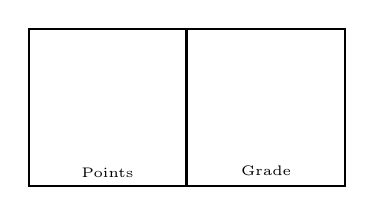
\begin{tikzpicture}[thick]
		\node (points) at (0,0) [draw,minimum size=2cm] {};
		\node (lbl-points) at (points.south) [anchor=south,font=\tiny] {Points};
		\node (grade) at (points.east) [draw,minimum size=2cm,anchor=west,
			outer sep=0] {};
		\node (lbl-grade) at (grade.south) [anchor=south,font=\tiny] {Grade};
	\end{tikzpicture}

	\begin{flushright}

		% Update this with your team number
		\huge\bfseries
		Team: 15 \\[1em]

		% Update this with your matriculation number, first name, second name
		\large
		01429540 Dinka MILOVANCEV \#1	\\
		01225461 Benedikt TUTZER \#2	\\
	
	\end{flushright}

	\vspace{5em}

	\begin{center}
		{\huge Digital Integrated Circuits Lab (LDIS)}\\[1em]
		{\Large 384.088, Summer Term 2018} \\[2em]
		{\large Supervisors:\\[.5em]
			Christian Krieg, Martin Mosbeck, Axel Jantsch} \\[10em]

		{\Huge Task 2: Blake2b cryptographic hash function
		}\\[10em]
	\end{center}


\begin{abstract}

		The task of our group was to implement \emph{BLAKE2b} hash function as specified in \autocite{rfc7693}. The \emph{BLAKE2b} algorithm computation was implemented using state machines, the implementation was syntactically correct and synthesizable. The functional correctness was verified by using the reference implementation given in C. The test bench compared the output of our entity with the reference hash value for the same message input and reported the result in terminal. For the message input we used the random data generated by the Task 1 implementation. The \emph{BLAKE2b} hash function entity is to be used as a component of \emph{Argon2} memory hard function which should generate cryptographically secure keys from passwords as specified in \autocite{irtf-cfrg-argon2-03}. The \emph{Argon2} function should be implemented targeting \emph{Nexyx 4 DDR} board.
\end{abstract}
\end{titlepage}
\pagenumbering{arabic}
%
%----------------------------------------------------------------------------
%
\section{Problem statement and motivation}
\label{sec:problem}
\emph{BLAKE2} hash function comes in two variants: \emph{BLAKE2b} for 64-bit platforms and \emph{BLAKE2s} for smaller architectures. \emph{BLAKE2b} hash function was implemented in this task based on \autocite{rfc7693}; the function is intended to be used in \emph{Argon2} memory-hard function for password hashing \autocite{irtf-cfrg-argon2-03} which is to be implemented in hardware targeting the \emph{Nexys 4 DDR} board. The final output of the \emph{Argon2} should be cryptographically secure key derived from the input password.
	
The input of the \emph{BLAKE2b} hash function is the message data (message length goes from 1 to $2^{128}$ bytes) and the output is the message digest or simply hash value (hash length goes from 1 to 64 bytes). According to the reference algorithm the input message is divided into $N$ 128 byte message blocks $m_i$; if the secret key is used then it is set as the first message block. In our design specification the secret key is not being used.

The hash value is iteratively computed as in the following pseudo-code:

\begin{algorithm}

	\ $h^{0}=IV$: initialization of the hash state vector with initialization vector IV (obtained by taking the first 64 bits of the fractional parts of the square roots of the first eight prime numbers)
	\BlankLine
	
    \For{$i:=0$ \textbf{to} $N$–2 }{
	$h^{i+1}$ $=$ \textbf{compress}($h_i, m_i,t_i,f=FALSE $); the compression function completely compresses one data block; it takes as an input previous hash states, current message block $m_i$ (divided into 16 words with length $w=$64 bit), 2$\cdot w $ offset counter $t_i$ that counts how many bytes have been compressed, and flag indicator $f$ for the last message block. The input message block is mixed into the current hash states.}
	
	\BlankLine
	\ $h^{N}$ $=$ ($h_{N-1}, m_{N-1},t_{N-1}$, $f=TRUE $), \textbf{ return $h^{N}$ } : computation of the final message block, the output is the first $hash\_len$ bytes of little endian state vector $h$. The input hash length parameter $hash\_len$ is in the range from 1 to 64 bytes.
	
	\caption{\emph{BLAKE2b} algorithm}
	\label{alg:bbs}
	
\end{algorithm}

The main challenge in implementing the algorithm is the compression function which is called for each message block. The mixing of the message block is done in 12 rounds, in each round message word schedule is defined by 10 possible permutations $\sigma$0…$\sigma$9 (hard coded into design as two dimensional SIGMA–array). The mixing of the messages requires additional mixing function which mixes two 64 bit words from the message $m_i$ into the hash state $h_i$. The auxiliary local 4$\times$4 working vector $v[0..15]$ is used for mixing function:
\[
   v=
  \left[ {\begin{array}{cccc}
   v_0 & v_1 &v_2 & v_3 \\
   v_4 & v_5 &v_6 & v_7\\
   v_8 & v_9 &v_{10} & v_{11}\\
   v_{12} & v_{13} &v_{14} & v_{15}
  \end{array} } \right]
\]
	    
Hash functions are used in various security protocols to ensure the integrity of the transmitted data. The transmitted data is mapped to a hash value $h$ of fixed size; it should be computationally impossible that two sets of data result in the same hash value or that a small change in message data does not result in a change in $h$, and it should be computationally impossible to reconstruct the input data from the hash value. The quality of our implementation of \emph{BLAKE2b} hash function is verified by using the reference C source code given in \autocite{rfc7693}.


%
%Briefly introduce your task here, state the problem and outline why it is
%important to solve this problem. Use \texttt{\textbackslash{}autocite}
%to cite any external reference, for example a
%survey\autocite{Petura2016} on \gls{fpga}-based \glspl{trng}. Use
%\emph{biber} to create the bibliography. \emph{JabRef}\autocite{JabRef} is
%a good graphical frontend to maintain your bibliography. Use the commands
%provided by the \texttt{\textbackslash{}glossaries} package to typeset
%acronyms, like \gls{trng} and \gls{fpga}. This will help you in consistently
%introducing and using abbreviations and acronyms.
%
%----------------------------------------------------------------------------
%
\section{Implementation (proposed solution)}
\label{sec:solution}
The algorithm for \emph{BLAKE2b} hash function was broken down into several main operations and coded in VHDL as a state machine. The states were the following:
\begin{itemize}
	\item \textbf{STATE_IDLE}: initialization of the \emph{BLAKE2b} hash function i.e. initial values for the hash state vector $h[0..7]$ (array of 8 64-bit values). If there is a new block message to be compressed the flag input bit $valid\_in$ is set to high, the next state is STATE_PREPARE. The counter of the compressed bytes ($compressed\_bytes$) is increased for 128, or if it is the last message block, the compressed bytes counter is set to total message length.
	\item \textbf{STATE_PREPARE}: initialization for \textbf{compress} function - the local state vector $v[0..15]$ is initialized with hash state vector $h[0..7]$ mixed with the number of received bytes, the counter $ci\_done$ for the mixing rounds is reset to zero (there should be 12 rounds for message mixing), the nest state is STATE_COMPRESS.
	\item \textbf{STATE_COMPRESS}: resets the counter for the mixing function $mi\_done$ to zero (maximum value 7), the next state is the first mixing state. At the end of the mixing states all the columns and diagonals of the working vector $v[0..15]$ will be mixed with words of the current message block. The first mixing state is STATE_MIX_A
	\item \textbf{STATE_MIX_A}: the first mixing state is one part of the implementation of mixing function G from \autocite{rfc7693} which requires additions of words. In each cycle one of the working vector $v[0..15]$ values is  computed depending on the SIGMA permutation constant, current mixing round and $mio\_left$ 2-bit tag which serves for internal codification of the mixing equations. The next mixing state is STATE_MIX_B.
	\item \textbf{STATE_MIX_B}:  the second mixing state is the second part of the implementation of mixing function G which requires xor operation and bit shifting. Again, in each cycle one of the working vector $v[0..15]$ values is  computed depending on the SIGMA permutation constant, current mixing round and internal $mio\_left$ 2-bit tag which serves for internal codification of the mixing equations. The $mio\_left$ is updated after each mixing $B$ operation. If there are still mixing operations to be done in a given round ($mi\_done \neq 7$) then the next state is STATE_MIX_A. There are in total 8 mixing operations ($mi\_done$) divided in states $A$ and $B$, and four operation codes ($mio\_left$) for $AB$ pairs. When all the codes are computed in a given order, the mixing code counter ($mio\_left$) is incremented. If the last mixing operation is done but there are still mixing rounds to be computed the next state is STATE_COMPRESS and rounds counter $ci\_done$ is updated. If all the mixing rounds are computed ($ci\_done = 11$), and the last message bit is sent ($seen\_last$ is high) the next state is STATE_DONE. If the last block message is still not sent but all the mixing rounds are computed the next state is STATE_MIX_H.
	\item \textbf{STATE_MIX_H}: mixing of the upper $v[0..7]$ and lower half $v[8..15]$ of the working vector $v[0..15]$ into the current state vector $h[0..7]$. The next state is the STATE_WAIT for the next message block to be compressed.
	\item \textbf{STATE_WAIT}: expecting the following message block, if received $valid\_in$ goes  high, the system variables are updated and the next state is STATE_PREPARE.
	\item \textbf{STATE_DONE}: when the last message block has been compressed, the hash output is computed. Next state is STATE_IDLE in which we wait the next message input.

	      \end{itemize}		
The operations described above can be seen in \Cref{code:sampling}.

\enlargethispage{-\baselineskip}
\begin{lstlisting}[
	style = vhdl,
	caption = {VHDL implementation of the \emph{BLAKE2b} hash function},
	label = {code:sampling},
]

process(clk, reset)
	--help variables for the mixing operations. These correspond
	--to the variable names in the paper
	variable a : std_logic_vector(63 downto 0);
	variable b : std_logic_vector(63 downto 0);
	variable c : std_logic_vector(63 downto 0);
	variable d : std_logic_vector(63 downto 0);
	variable x : std_logic_vector(63 downto 0);
	variable y : std_logic_vector(63 downto 0);
	variable help_sigma_x : integer range 0 to 15;
	variable help_sigma_y : integer range 0 to 15;
	begin
		if reset = '1' then
			state <= STATE_IDLE;
			current_chunk <= (others => '0');
			seen_last <= '0';
			compress_ready <= '1';
			h <= (others => (others => '0'));
			v <= (others => (others => '0'));
			compressed_bytes <= (others => '0');
			mio_left <= "00";
			valid_out <= '0';
			hash <= (others => '0');
		elsif rising_edge(clk) then
			--assign the right local vector and message to the variables
			--according to the index table
			a := v(ind(mi_done, 0));
			b := v(ind(mi_done, 1));
			c := v(ind(mi_done, 2));
			d := v(ind(mi_done, 3));
			help_sigma_x := SIGMA(ci_done, ind(mi_done,4));
			x := current_chunk(help_sigma_x*64+63 downto help_sigma_x*64);
			help_sigma_y := SIGMA(ci_done, ind(mi_done,5));
			y := current_chunk(help_sigma_y*64+63 downto help_sigma_y*64);

			case(state) is
				when STATE_IDLE =>
					--initialize the persistent state vector
					h(1 to 7) <= VI(1 to 7);
					h(0) <= VI(0) xor (X"00000000010100" &
						std_logic_vector(
						to_unsigned(hash_len, 8)));
					--no bytes yet received
					if valid_in = '1' then
						--if a message chunk is received, it is saved together
						--with all inputs and the state machine moves to the
						--prepare state
						state <= STATE_PREPARE;
						current_chunk <= message;
						seen_last <= last_chunk;
						ci_done <= 0;
						compress_ready <= '0';
						total_bytes <= message_len;
						--if this was the last chunk, the number of received
						--bytes is equal to the length of the received message.
						--Otherwise it is increased by 128.
						if last_chunk = '1' then
							compressed_bytes <= std_logic_vector(
								to_unsigned(message_len, 128));
						else
							compressed_bytes <= std_logic_vector(
								unsigned(compressed_bytes) + 128);
						end if;
						--the entity is not ready to receive new input
						valid_out <= '0';
					end if;
				when STATE_PREPARE =>
					--the persistent state vector is copied onto the local
					--state vector
					for i in 0 to 7 loop
						V(i) <= h(i);
					end loop;
					V(8) <= VI(0);
					V(9) <= VI(1);
					V(10) <= VI(2);
					V(11) <= VI(3);
					--the number of received bytes is mixed into the vector
					V(12) <= VI(4) xor compressed_bytes(63 downto 0);
					V(13) <= VI(5) xor compressed_bytes(127 downto 64);
					--inverted if the last chunk is sent
					if seen_last = '1' then
						V(14) <= not VI(6);
					else
						V(14) <= VI(6);
					end if;
					V(15) <= VI(7);
					--reset the counter for the compression stage
					ci_done <= 0;
					--move on to the compress state
					state <= STATE_COMPRESS;

				when STATE_WAIT =>
					--a subsequent message chunk was received (not the first)
					if valid_in = '1' then
						state <= STATE_PREPARE;
						current_chunk <= message;
						seen_last <= last_chunk;
						compress_ready <= '0';
						if last_chunk = '1' then
							compressed_bytes <= std_logic_vector(
								to_unsigned(total_bytes,128));
						else
							compressed_bytes <= std_logic_vector(
								unsigned(compressed_bytes) + 128);
						end if;
					end if;

				when STATE_COMPRESS =>
					--reset the counter for the mixing stage
					mi_done <= 0;
					--start mixing
					state <= STATE_MIX_A;
				when STATE_MIX_A =>
					--additions as defined by blake2b
					case mio_left is
						when "11"|"01" =>
					v(ind(mi_done, 2)) <= std_logic_vector(
						unsigned(c)+unsigned(d));
						when "00" =>
					v(ind(mi_done, 0)) <= std_logic_vector(
						unsigned(a)+unsigned(b)+unsigned(x));
						when "10" =>
					v(ind(mi_done, 0)) <= std_logic_vector(
						unsigned(a)+unsigned(b)+unsigned(y));
						when others =>
					end case;

					state <= STATE_MIX_B;
				when STATE_MIX_B =>
					--xor's and shifts as defined by blake2b
					case mio_left is
						when "00" =>
					v(ind(mi_done,3)) <= std_logic_vector(
						unsigned(d xor a) ror 32);
						when "11" =>
					v(ind(mi_done,1)) <= std_logic_vector(
						unsigned(b xor c) ror 24);
						when "10" =>
					v(ind(mi_done,3)) <= std_logic_vector(
						unsigned(d xor a) ror 16);
						when "01" =>
					v(ind(mi_done,1)) <= std_logic_vector(
						unsigned(b xor c) ror 63);
						when others =>
					end case;

					--last mix
					if mi_done = 7 and mio_left = "01" then
						--also last compression
						if ci_done = 11 then
							--also last chunk
							if seen_last = '1' then
								state <=
								STATE_DONE;
							else
								state <=
								STATE_MIX_H;
							end if;
							--ready to receive a new chunk
							compress_ready <= '1';
						else
							--next compression
							state <= STATE_COMPRESS;
							ci_done <=
								ci_done + 1;
						end if;
					else
						if mio_left = "01" then
							mi_done <=
								mi_done +1;
						end if;
						state <= STATE_MIX_A;
					end if;
					mio_left <= std_logic_vector(unsigned(mio_left) + 3);
				when STATE_DONE =>
					--write output
					for i in 0 to 7 loop
						hash(i*64+63 downto i*64) <= h(i) xor v(i) xor v(i+8);
					end loop;
					valid_out <= '1';
					compressed_bytes <= (others => '0');
					state <= STATE_IDLE;
				when STATE_MIX_H =>
					state <= STATE_WAIT;
					--mix into h
					for i in 0 to 7 loop
						h(i) <= h(i) xor v(i) xor v(i+8);
					end loop;
				when others =>
					state <= STATE_IDLE;
			end case;
		end if;
	end process;

\end{lstlisting}

%\lipsum[2]
%
%----------------------------------------------------------------------------
%
\section{Results (verification plan)}
\label{sec:results}

In order to verify the proper operation of the implemented \emph{BLAKE2b} hash function, a test bench was made that uses as an input \texttt{messages.txt} file. The content of this file is the input data to be hashed. The same input data is being used by the reference C code \autocite{rfc7693} which computes its output hash values into the document \texttt{hashes.txt}. In the test bench each line from the \texttt{messages.txt} is being read and the final hash values are computed by using our VHDL implementation. These values are then compared with the results of implementation in the reference C code stored in the document \texttt{hashes.txt}. In order to read the hash values from \texttt{hashes.txt}, a conversion from \texttt{hexadecimal} to \texttt{std_logic_vector} was needed; the ASCII_2_STD function was used for this purpose. This can be seen in the \Cref{code:testing}.

\begin{lstlisting}[style = vhdl,caption = {Test bench process for verifying the hardware implementation using the reference implementation in C},label = {code:testing},]
stimuli : process
		type char_file_t is file of character;
		file message_file : TEXT open read_mode is "messages.txt";
		file hash_file : TEXT open read_mode is "hashes.txt";
		variable line_buffer : line;
		variable value_in : std_logic_vector(64*8-1 downto 0);
		variable char_value_1 : std_logic_vector(7 downto 0);
		variable char_value_2 : std_logic_vector(7 downto 0);
		variable read_ok : boolean;
		variable current_char : character;
		variable counter : integer;
	begin

		--always generate 64-byte hashes
		hash_len <= 64;
		last_chunk <= '0';

		--start with reset
		reset <= '1';
		wait for 10 ns;
		reset <= '0';
		wait for 5 ns;

		counter := 0;
		message <= (others => '0');
		while not endfile(message_file) loop
			counter := 0;
			message <= (others => '0');
			wait for period;

			--read single line
			readline(message_file, line_buffer);
			--message length equals line length
			message_len <= line_buffer'length;

			for i in 0 to line_buffer'length-1 loop
				--read one byte of data and write it to message
				--if message is filled up, send it to the entity
				--and start over
				if counter = 128 then
					wait for period;
					last_chunk <= '0';
					valid_in <= '1';
					wait for period;
					valid_in <= '0';

					counter := 0;
					message <= (others => '0');
					wait for period*835;
				end if;

				read(line_buffer, current_char);
				char_value_1 := std_logic_vector(to_unsigned(
					character'pos(current_char),8));
				message(counter*8+7 downto counter*8) <=
					char_value_1;
				counter := counter + 1;
			end loop;

			--send the remaining bytes as last chunk
			wait for period;
			last_chunk <= '1';
			valid_in <= '1';
			wait for period;
			valid_in <= '0';
			wait for period*835;

			readline(hash_file, line_buffer);
			--report "line " & line_buffer.all;
			
			--read hash file in hex and compare with the output
			--generated by the entity
			counter := 0;
			value_in := (others => '0');
			for i in 0 to 63 loop
				read(line_buffer, current_char);
				char_value_1 := std_logic_vector(to_unsigned(
					character'pos(current_char),8));
				read(line_buffer, current_char);
				char_value_2 := std_logic_vector(to_unsigned(
					character'pos(current_char),8));
				value_in(counter*8+7 downto counter*8) :=
					ASCII_2_VEC(char_value_1) &
					ASCII_2_VEC(char_value_2);
				counter := counter + 1;
			end loop;

			--report "valu " & to_hstring(value_in);
			--report "hash " & to_hstring(hash);

			if value_in = hash then
				report "[ OK] HASH correct";
			else
				report "[NOK] HASH incorrect";
			end if;
		end loop;

		ended <= '1';

		wait;
	end process;

\end{lstlisting}

The state transitions for the case when the next block message is to be received, together with the counters for mixing rounds and mixing operations, are shown in \Cref{signaling}. After the previous message block was compressed (round counter $ci\_done$ is 11, and the state is STATE_WAIT), as the new message block is available the $valid\_in$ goes high for one clock cycle, the $current\_chunk$ becomes the new message block, the state is STATE_PREPARE, and the message block register $message$ is freed. The following are the mixing  states, after each mixing $A$ and mixing $B$ pair the mixing code $mio\_left$ is updated. The compression of one message block takes 835 clock cycles.

  \begin{figure}[!ht]
	\centering
	\begin{tikzpicture}[
			circuit logic IEC,
			circuit ee IEC,
			x = 5cm, y = 2cm,
			every info/.style = {font = \scriptsize},
			set diode graphic = var diode IEC graphic,
			set make contact graphic = var make contact IEC graphic,
		]

		\node at (0,0) {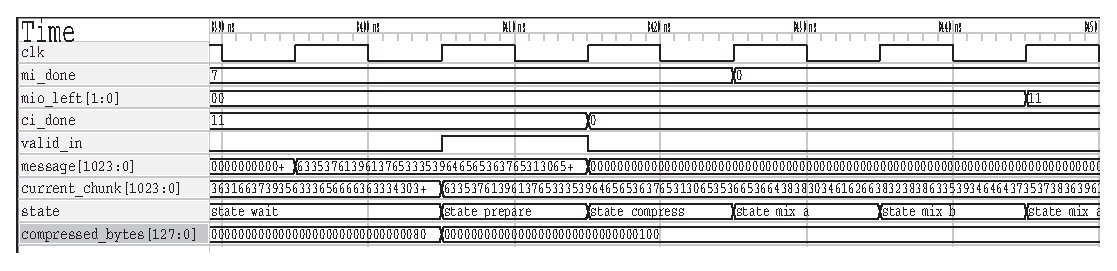
\includegraphics[scale=0.93]{waveform2.eps}};

	\end{tikzpicture}
	\caption{Simulation results for blake2b hash function: state transitions}
	\label{signaling}
\end{figure}

For the message data input we used the hexadecimal random data from Task 1 as 1032 byte input message. Additional  message was created by replacing only the first character with '1' in order to verify that even such a small change in input can lead to entirely different hash values. This can be seen in \Cref{2messagehash}. These hash values matched the hash values from the C code implementation.

\begin{figure}[!ht]
	\centering
	\begin{tikzpicture}[
			circuit logic IEC,
			circuit ee IEC,
			x = 5cm, y = 2cm,
			every info/.style = {font = \scriptsize},
			set diode graphic = var diode IEC graphic,
			set make contact graphic = var make contact IEC graphic,
		]

		\node at (0,0) {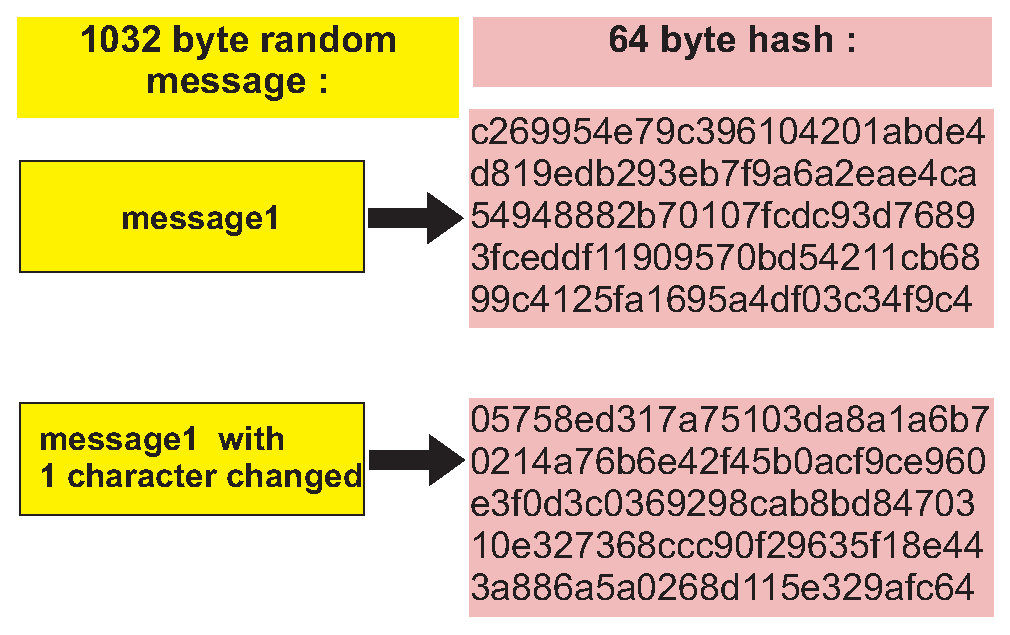
\includegraphics[scale=0.52]{hashmessage.eps}};

	\end{tikzpicture}
	\caption{Similar input data results in a very different hash messages}
	\label{2messagehash}
\end{figure}

Since this design is to be used as a module of the larger \emph{Argon2} design, there were no ports to be mapped to the hardware and therefore placing and routing of the design was not possible, but the RTL synthesis and optimization was successfully completed. The RTL optimization report is shown in  \Cref{RTLsynthesis}.

\begin{lstlisting}[
	style = vhdl,
	caption = {RTL Hierarchical Component Statistics},
	label = {RTLsynthesis},
]
-
Hierarchical RTL Component report 
Module blake2b 
Detailed RTL Component Info : 
+---Adders : 
	   2 Input    128 Bit       Adders := 1     
	   3 Input     64 Bit       Adders := 1     
	   2 Input      4 Bit       Adders := 1     
	   2 Input      3 Bit       Adders := 1     
	   2 Input      2 Bit       Adders := 1     
+---XORs : 
	   2 Input     64 Bit         XORs := 5     
	   3 Input     64 Bit         XORs := 8     
+---Registers : 
	             1024 Bit    Registers := 1     
	              512 Bit    Registers := 1     
	              128 Bit    Registers := 1     
	               64 Bit    Registers := 24    
	               11 Bit    Registers := 1    
	                4 Bit    Registers := 1     
	                3 Bit    Registers := 2     
	                2 Bit    Registers := 1     
	                1 Bit    Registers := 3     
+---Muxes : 
	   8 Input    128 Bit        Muxes := 1     
	   2 Input    128 Bit        Muxes := 2     
	   3 Input     64 Bit        Muxes := 3     
	   8 Input     64 Bit        Muxes := 23    
	   4 Input     64 Bit        Muxes := 1     
	   9 Input     64 Bit        Muxes := 1     
	   8 Input      4 Bit        Muxes := 11    
	   8 Input      3 Bit        Muxes := 11    
	   2 Input      3 Bit        Muxes := 1     
	   3 Input      3 Bit        Muxes := 1     
	   8 Input      1 Bit        Muxes := 17    
	  11 Input      1 Bit        Muxes := 12    
	   4 Input      1 Bit        Muxes := 16    
	   2 Input      1 Bit        Muxes := 27    
----------------------------------------------
Finished RTL Hierarchical Component Statistics
----------------------------------------------

\end{lstlisting}



%
%----------------------------------------------------------------------------
%
\section{Discussion}
\label{sec:discussion}
In the reference paper \autocite{rfc7693} for \emph{BLAKE2b} hash function coded in C, the input parameter was the whole message that can have between 1 and $2^{128}$ bytes. This long message was intended to be divided into 128-byte message blocks during computing. Since the VHDL cannot support such large input vectors we decided to send the message block by block. In this way our data input is 128 bytes long and we have additional information about the message length ($message\_len$). The maximum message length was specified to be 1032 bytes since this is the maximum length needed by \emph{Argon2}. For every message block we need the information of the main module whether there is a new message block available (signal $valid\_in$ goes high) and the flag register for the last message block $last\_chunk$ (high if the last message block is sent). As the output we provide handshaking signals $compress\_ready$ and $valid\_out$, the user of our entity must make sure that $compress\_ready$ is high before sending a new message block, and the output i.e. the hash can be stored when $valid\_out$ is high.

The input messages in \texttt{messages.txt} file can be empty message. However messages are not allowed to contain whitespaces.
%----------------------------------------------------------------------------
%
\section{Conclusions}
\label{sec:conclusions}

In this task we implemented \emph{BLAKE2b} hash algorithm in the hardware. The design was synthesizable, however the final utilization report can be done once the entity module is used inside the \emph{Argon2} implementation, when it will be mapped to the target hardware (\emph{Nexys 4 DDR}). 

The functional verification of our design was performed through simulation. The random data was used as the message input and the reference implementation in C was used to validate that the correct hash output has been computed.
%
%----------------------------------------------------------------------------
%
\pagebreak
\section{Assessment}
\label{sec:assessment}

This is the place for the teaching staff to add notes for team assessment.

\begin{table}[h!]
	\centering
	\renewcommand{\arraystretch}{2}
	\begin{tabular}{
		|p{.025\linewidth}
		|p{.75\linewidth}
		|p{.05\linewidth}
		|p{.05\linewidth}|
	}

		\hline
		\textbf{\#} & \textbf{Issue} & \textbf{Yes} & \textbf{No} \\
		\hline

		\multicolumn{4}{|p{.95\linewidth}|}{\cellcolor{gray!20} 1 Implementation}
			\\\hline

		1.1 & Does the implementation conform to the specification? & & \\\hline

		1.2 & Is the implementation resource-efficient? & & \\\hline

		1.3 & Is the implementation's \gls{hdl} complexity low? & & \\\hline

		1.4 & Is the implementation well-documented? & & \\\hline

		1.5 & Is the file structure's complexity low? & & \\\hline

		\multicolumn{4}{|p{.95\linewidth}|}{\cellcolor{gray!20} 2 Coding style}
			\\\hline

		2.1 & Is the line width of code code limited to 80 characters?
			& & \\\hline

		2.2 & Is white space appropriately used? & & \\\hline

		2.3 & Are tabs used for indentation? & & \\\hline

		2.4 & Are separators used to logically divide the file contents? & & \\\hline

		2.5 & Are meaningful comments given? & & \\\hline

		\multicolumn{4}{|p{.95\linewidth}|}{\cellcolor{gray!20} 3 Code reuse} \\\hline

		3.1 & Is publicly available code re-used? & & \\\hline

		3.2 & Is non-publicly available code re-used? & & \\\hline

		3.3 & Are the sources of re-used code cited? & & \\\hline

		\multicolumn{4}{|p{.95\linewidth}|}{\cellcolor{gray!20} 4 Interaction}
			\\\hline

		4.1 & Was the specification unclear to the team? & & \\\hline

		4.2 & If yes, did the team contact the teaching staff to make the specification
			clear? & & \\\hline

		\multicolumn{4}{|p{.95\linewidth}|}{\cellcolor{gray!20} 5 Report}
			\\\hline

		5.1 & Are there typos? & & \\\hline

		5.2 & Is the report grammatically correct? & & \\\hline

		5.3 & Is there redundant information? & & \\\hline

		5.4 & Is the report's format consistent? & & \\\hline

		5.5 & Are captions properly used and numbered? Page numbers? & & \\\hline

		5.6 & Are figures and tables properly referenced in the body text?
			& & \\\hline

		5.7 & Are resources properly referenced? & & \\\hline

%		 & & & \\\hline

		\hline

	\end{tabular}
\end{table}
%
%----------------------------------------------------------------------------
%
% References
%
\printbibliography
%
%----------------------------------------------------------------------------
%

\end{document}
%
%----------------------------------------------------------------------------
